\documentclass[12pt,a4paper]{article}
\usepackage{fontspec}
\setmainfont{Times New Roman}[Path=C:/Windows/Fonts/,UprightFont=times.ttf,BoldFont=timesbd.ttf,ItalicFont=timesi.ttf,BoldItalicFont=timesbi.ttf]
\usepackage{amsmath,amssymb,amsfonts}
\usepackage[left=1.5cm,right=1.5cm,top=1.5cm,bottom=1.7cm,headheight=17pt]{geometry}
\usepackage{enumitem,array,graphicx,tikz,fancyhdr,needspace}
\usetikzlibrary{arrows.meta,calc,patterns}
\pagestyle{fancy}
\fancyhf{}
\lhead{\small\textbf{HƯỚNG TỚI THPTQG 2027}}
\rhead{\small\textit{Biên soạn: Dương Gia Bảo}}
\rfoot{\small Trang \thepage/5 - Mã đề: 0016}
\renewcommand{\headrulewidth}{0.4pt}
\fancypagestyle{firstpage}{\fancyhead{}\renewcommand{\headrulewidth}{0pt}}
\setlength{\parindent}{0pt}
\setlength{\parskip}{3pt}
\setlength{\emergencystretch}{1em}
\setlist[enumerate,1]{label=\textbf{Câu \arabic*:},leftmargin=*,itemsep=8pt,topsep=5pt}
\setlist[enumerate,2]{label=\alph*),leftmargin=*,itemsep=3pt,topsep=3pt}
\newcommand{\bonpa}[4]{\par\smallskip\noindent
\begin{tabular}{@{}p{0.47\linewidth}p{0.47\linewidth}@{}}
\textbf{A.} #1 & \textbf{B.} #2\\[3pt]
\textbf{C.} #3 & \textbf{D.} #4\end{tabular}}
\newcommand{\loigiai}[1]{\par\medskip\Needspace{4\baselineskip}\noindent\textbf{#1}\par\nobreak}
\begin{document}
\thispagestyle{firstpage}
\noindent
\begin{minipage}[t]{0.35\textwidth}
    \centering
    {\fontsize{13}{15}\selectfont\textbf{HƯỚNG TỚI THPTQG 2027}}\\[5pt]
    \textit{Biên soạn: Dương Gia Bảo}\\[6pt]
    \setlength{\fboxrule}{0.8pt}%
    \setlength{\fboxsep}{5pt}%
    \fbox{\begin{minipage}{0.83\linewidth}
        \centering
        {\fontsize{13}{15}\selectfont\textbf{ĐỀ ÔN TẬP}\\[2pt]\textbf{CHÍNH THỨC}}\\[5pt]
        \textit{(Đề thi gồm có 05 trang)}
    \end{minipage}}
\end{minipage}\hfill
\begin{minipage}[t]{0.63\textwidth}
    \centering
    {\fontsize{13}{15}\selectfont\textbf{KỲ KHẢO SÁT CHẤT LƯỢNG LỚP 12}\\[2pt]
    \textbf{NĂM HỌC 2026 - 2027}}\\[6pt]
    {\fontsize{14}{16}\selectfont\textbf{Môn: TOÁN - Lớp 12 (ĐỀ SỐ 16)}}\\[5pt]
    {\fontsize{11.5}{13}\selectfont\textit{Thời gian làm bài: 90 phút, không kể thời gian giao đề}}\\[6pt]
    \setlength{\fboxrule}{0.8pt}%
    \setlength{\fboxsep}{6pt}%
    \fbox{\makebox[3cm]{\fontsize{14}{16}\selectfont\textbf{Mã đề: 0016}}}
\end{minipage}
\par\vspace{3pt}
\hrule height 0.6pt
\vspace{4pt}
\noindent\textit{Họ và tên học sinh:}\dotfill\hspace{1cm}\textit{Lớp:}\makebox[3.5cm]{\dotfill}
\par\vspace{3pt}
\hrule height 0.6pt
\vspace{4pt}

\section*{\large PHẦN I. CÂU TRẮC NGHIỆM NHIỀU PHƯƠNG ÁN LỰA CHỌN}
\textit{Thí sinh trả lời từ câu 1 đến câu 12. Mỗi câu thí sinh chỉ chọn một phương án. Mỗi câu trả lời đúng được 0,25 điểm.}

\begin{enumerate}
\item Cho hàm số $y = -x^3 + 3x^2 - 4$. Hàm số đã cho đồng biến trên khoảng nào dưới đây?
\bonpa{$(0; 2)$.}{$(-\infty; 0)$.}{$(2; +\infty)$.}{$(-1; 3)$.}

\item Cho hàm số $y = \dfrac{x^2 - 3x + 6}{x - 1}$. Giá trị cực tiểu của hàm số đã cho bằng
\bonpa{$-5$.}{$3$.}{$-1$.}{$5$.}

\item Đường tiệm cận xiên của đồ thị hàm số $y = \dfrac{2x^2 - 3x + 5}{x + 1}$ có phương trình là
\bonpa{$y = 2x + 5$.}{$y = 2x - 3$.}{$y = 2x - 5$.}{$y = x - 5$.}

\item Nghiệm của phương trình $\log_2(3x - 1) = 3$ là
\bonpa{$x = \dfrac{7}{3}$.}{$x = \dfrac{10}{3}$.}{$x = 1$.}{$x = 3$.}

\item Họ tất cả các nguyên hàm của hàm số $f(x) = 3x^2 + 2\sin x$ là
\bonpa{$x^3 - 2\cos x + C$.}{$x^3 + 2\cos x + C$.}{$6x - 2\cos x + C$.}{$x^3 + 2\sin x + C$.}

\item Cho $\displaystyle\int_1^3 f(x)\,\mathrm{d}x = 4$ và $\displaystyle\int_1^3 g(x)\,\mathrm{d}x = -2$. Khi đó $\displaystyle\int_1^3 [2f(x) - 3g(x)]\,\mathrm{d}x$ bằng
\bonpa{$2$.}{$14$.}{$6$.}{$10$.}

\item Trong không gian $Oxyz$, cho hai điểm $A(1; 2; -1)$ và $B(3; 0; 5)$. Tọa độ trung điểm $M$ của đoạn thẳng $AB$ là
\bonpa{$(4; 2; 4)$.}{$(1; -1; 3)$.}{$(2; 1; 2)$.}{$(2; -1; 3)$.}

\item Trong không gian $Oxyz$, mặt cầu $(S): x^2 + y^2 + z^2 - 2x + 4y - 6z + 5 = 0$ có bán kính bằng
\bonpa{$9$.}{$\sqrt{5}$.}{$\sqrt{19}$.}{$3$.}

\item Khảo sát thời gian tự học mỗi ngày (đơn vị: giờ) của $40$ học sinh thu được bảng số liệu ghép nhóm sau:
\begin{center}
\begin{tabular}{|c|c|c|c|c|}\hline
Thời gian & $[0; 1)$ & $[1; 2)$ & $[2; 3)$ & $[3; 4)$\\\hline
Số học sinh & $6$ & $14$ & $12$ & $8$\\\hline
\end{tabular}
\end{center}
Thời gian tự học trung bình của mẫu số liệu ghép nhóm này bằng
\bonpa{$2{,}05$ giờ.}{$2{,}15$ giờ.}{$1{,}95$ giờ.}{$2{,}20$ giờ.}

\item Một hộp chứa $10$ quả bóng bàn gồm $6$ quả màu trắng và $4$ quả màu vàng. Lấy ngẫu nhiên lần lượt hai quả bóng (không hoàn lại). Biết rằng quả bóng lấy ra ở lần thứ nhất có màu trắng, xác suất để quả bóng lấy ra ở lần thứ hai cũng có màu trắng bằng
\bonpa{$\dfrac{3}{5}$.}{$\dfrac{5}{9}$.}{$\dfrac{1}{3}$.}{$\dfrac{2}{9}$.}

\item Trong không gian $Oxyz$, khoảng cách từ điểm $A(1; -2; 3)$ đến mặt phẳng $(P): 2x - 2y + z + 3 = 0$ bằng
\bonpa{$3$.}{$\dfrac{10}{3}$.}{$4$.}{$2$.}

\item Cho cấp số nhân $(u_n)$ có số hạng đầu $u_1 = 3$ và công bội $q = 2$. Tổng của $6$ số hạng đầu tiên $S_6$ bằng
\bonpa{$192$.}{$93$.}{$381$.}{$189$.}
\end{enumerate}

\newpage
\section*{\large PHẦN II. CÂU TRẮC NGHIỆM ĐÚNG SAI}
\textit{Thí sinh trả lời từ câu 1 đến câu 4. Trong mỗi ý a), b), c), d) ở mỗi câu, thí sinh chọn đúng hoặc sai. Ở mỗi câu, thí sinh chỉ chọn chính xác 1 ý được 0,1 điểm; chỉ chọn chính xác 2 ý được 0,25 điểm; chỉ chọn chính xác 3 ý được 0,5 điểm; chọn chính xác cả 4 ý được 1,0 điểm.}

\begin{enumerate}
\item Một doanh nghiệp sản xuất một loại thiết bị gia dụng. Khi sản xuất và bán $x$ nghìn thiết bị ($0 < x \le 15$), hàm tổng chi phí được cho bởi $C(x) = x^3 - 12x^2 + 72x + 100$ (trăm triệu đồng). Giá bán mỗi nghìn thiết bị phụ thuộc vào lượng cung theo hàm giá $p(x) = 120 - 3x$ (trăm triệu đồng). Giả sử toàn bộ sản phẩm sản xuất ra đều được bán hết.
\begin{enumerate}
\item Hàm tổng doanh thu của doanh nghiệp là $R(x) = 120x - 3x^2$ (trăm triệu đồng).
\item Doanh thu biên của doanh nghiệp tại mức sản lượng $x = 5$ nghìn thiết bị là $80$ trăm triệu đồng.
\item Doanh nghiệp đạt lợi nhuận lớn nhất khi mức sản lượng bằng $8$ nghìn thiết bị.
\item Mức lợi nhuận lớn nhất của doanh nghiệp bằng $348$ trăm triệu đồng.
\end{enumerate}

\item \begin{minipage}[t]{0.56\linewidth}
Trong không gian $Oxyz$ (đơn vị: kilômét), một trạm điều phối không lưu đặt tại gốc tọa độ $O(0; 0; 0)$ có vùng phủ sóng radar là một khối cầu bán kính $50\text{ km}$. Một chiếc máy bay di chuyển thẳng đều với vận tốc $480\text{ km/h}$, quỹ đạo là đường thẳng $d$ đi qua điểm $A(20; 10; 20)$ và có vectơ chỉ phương $\vec{u} = (2; -2; -1)$.
\begin{enumerate}
\item Mặt cầu giới hạn vùng phủ sóng radar của trạm có phương trình $x^2 + y^2 + z^2 = 2500$.
\item Khoảng cách ngắn nhất từ trạm radar $O$ đến đường bay của máy bay bằng $30\text{ km}$.
\item Điểm $B(26; 4; 17)$ không thuộc đường bay của máy bay.
\item Thời gian máy bay di chuyển trong vùng phủ sóng của trạm radar là $12$ phút.
\end{enumerate}
\end{minipage}\hfill
\begin{minipage}[t]{0.41\linewidth}
\vspace{-0.3\baselineskip}
\centering
\resizebox{\linewidth}{!}{%
\begin{tikzpicture}[>=Stealth, line cap=round, line join=round, font=\large]
\fill[teal!8] (0,0) circle (2.8);
\draw[teal!70!black, thick] (0,0) circle (2.8);
\draw[->, blue!65!black, very thick] (-3.8,1.68) -- (3.8,1.68) node[right, black] {$d$};
\draw[dashed, thick] (0,0) -- (0,1.68) node[midway, right] {$30$};
\draw[thick] (0,1.45) -- (0.23,1.45) -- (0.23,1.68);
\draw[dashed, thick] (0,0) -- (2.236,1.68);
\node[above] at (1.1,0.9) {$50$};
\fill (0,0) circle (2.5pt) node[below left] {$O$};
\fill (0,1.68) circle (2.5pt) node[above left] {$H$};
\fill (-2.236,1.68) circle (2pt) node[above left] {$M_1$};
\fill (2.236,1.68) circle (2pt) node[above right] {$M_2$};
\node at (0,-2.3) {\small Vùng phủ sóng radar};
\end{tikzpicture}%
}
\end{minipage}

\item Một bệnh viện thực hiện xét nghiệm tầm soát một loại bệnh cho nhóm người đến khám. Theo thống kê dịch tễ, tỉ lệ người thực sự mắc bệnh này trong nhóm người đến khám là $4\%$. Kỹ thuật xét nghiệm có độ chính xác như sau:
\begin{itemize}[leftmargin=*,itemsep=2pt,topsep=2pt]
\item Đối với người mắc bệnh, xác suất xét nghiệm cho kết quả dương tính là $95\%$.
\item Đối với người không mắc bệnh, xác suất xét nghiệm cho kết quả dương tính giả là $5\%$.
\end{itemize}
Chọn ngẫu nhiên một người trong nhóm đến khám để làm xét nghiệm.
\begin{enumerate}
\item Xác suất để người được chọn có kết quả xét nghiệm dương tính là $0{,}086$.
\item Xác suất để người được chọn không mắc bệnh và có kết quả xét nghiệm âm tính là $0{,}912$.
\item Biết người được chọn có kết quả xét nghiệm âm tính, xác suất người đó thực sự mắc bệnh lớn hơn $0{,}01$.
\item Trong số những người có kết quả xét nghiệm dương tính, tỉ lệ người thực sự mắc bệnh nhỏ hơn $50\%$.
\end{enumerate}

\item \begin{minipage}[t]{0.56\linewidth}
Một khuôn viên hình chữ nhật $ABCD$ có chiều dài $AB = 6\text{ m}$ và chiều rộng $AD = 4\text{ m}$. Người ta thiết kế một bồn hoa được giới hạn bởi một đường cong parabol có đỉnh là trung điểm của cạnh $CD$ và đi qua hai điểm $A, B$. Phần đất giới hạn bởi parabol và đoạn thẳng $AB$ là phần đất trồng hoa (phần gạch chéo), phần còn lại của hình chữ nhật được lát gạch men (phần để trắng).
\begin{enumerate}
\item Trong hệ trục tọa độ $Oxy$ với gốc $O$ là trung điểm của $AB$, parabol có phương trình $y = -\dfrac{4}{9}x^2 + 4$.
\item Diện tích phần đất dùng để trồng hoa bằng $18\text{ m}^2$.
\item Tỉ số giữa diện tích phần đất trồng hoa và diện tích phần lát gạch bằng $2$.
\item Chi phí trồng hoa là $150\,000$ đồng/m$^2$ và chi phí lát gạch là $250\,000$ đồng/m$^2$. Tổng chi phí hoàn thiện toàn bộ mảnh đất là $4{,}4$ triệu đồng.
\end{enumerate}
\end{minipage}\hfill
\begin{minipage}[t]{0.41\linewidth}
\vspace{-0.3\baselineskip}
\centering
\resizebox{\linewidth}{!}{%
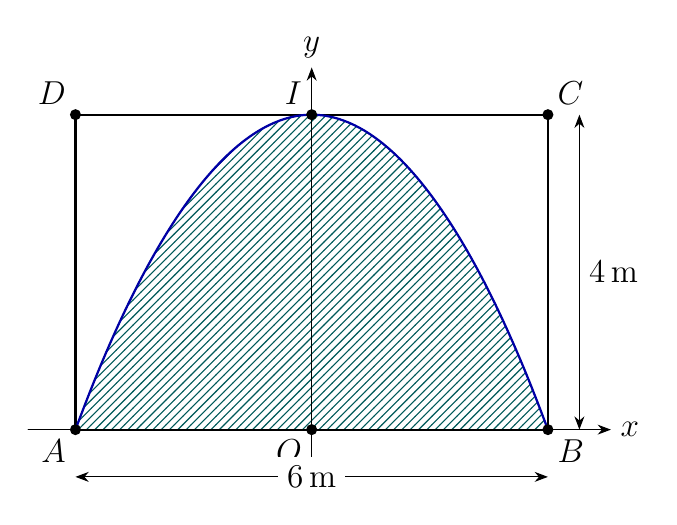
\begin{tikzpicture}[>=Stealth, line cap=round, line join=round, font=\large]
\draw[thick] (-3,0) rectangle (3,4);
\draw[pattern=north east lines, pattern color=teal!70!black] (-3,0) parabola bend (0,4) (3,0) -- cycle;
\draw[thick, blue!65!black] (-3,0) parabola bend (0,4) (3,0);
\draw[->] (-3.6,0) -- (3.8,0) node[right] {$x$};
\draw[->] (0,-0.5) -- (0,4.6) node[above] {$y$};
\fill (-3,0) circle (2pt) node[below left] {$A$};
\fill (3,0) circle (2pt) node[below right] {$B$};
\fill (3,4) circle (2pt) node[above right] {$C$};
\fill (-3,4) circle (2pt) node[above left] {$D$};
\fill (0,4) circle (2pt) node[above left] {$I$};
\fill (0,0) circle (2pt) node[below left] {$O$};
\draw[<->] (-3,-0.6) -- (3,-0.6) node[midway, fill=white] {$6\,\mathrm{m}$};
\draw[<->] (3.4,0) -- (3.4,4) node[midway, fill=white, right] {$4\,\mathrm{m}$};
\end{tikzpicture}%
}
\end{minipage}
\end{enumerate}

\Needspace{8\baselineskip}
\section*{\large PHẦN III. CÂU TRẮC NGHIỆM TRẢ LỜI NGẮN}
\textit{Thí sinh trả lời từ câu 1 đến câu 6. Mỗi câu trả lời đúng được 0,5 điểm. Chỉ làm tròn ở kết quả cuối cùng.}

\begin{enumerate}
\item Điểm kiểm tra học kỳ môn Toán của $50$ học sinh được thống kê theo các nhóm điểm trong bảng sau, trong đó $x$ và $y$ là hai tần số chưa biết:
\begin{center}
\resizebox{0.95\linewidth}{!}{%
\begin{tabular}{|l|c|c|c|c|c|c|}\hline
Khoảng điểm & $[4; 5)$ & $[5; 6)$ & $[6; 7)$ & $[7; 8)$ & $[8; 9)$ & $[9; 10)$\\\hline
Số học sinh & $6$ & $12$ & $x$ & $y$ & $8$ & $4$\\\hline
\end{tabular}%
}
\end{center}
Biết điểm trung bình của mẫu số liệu ghép nhóm bằng $6{,}82$. Tứ phân vị thứ ba $Q_3$ của mẫu số liệu ghép nhóm bằng bao nhiêu? \textit{(Làm tròn kết quả đến hàng phần trăm.)}

\item \begin{minipage}[t]{0.70\linewidth}
Trong loạt sút luân lưu 11m của một trận chung kết bóng đá, một cầu thủ thực hiện các lượt sút phạt đền. Theo thống kê, xác suất anh thực hiện thành công quả phạt đền đầu tiên là $0{,}85$. Ở các quả tiếp theo, nếu quả sút ngay trước đó thành công thì xác suất sút thành công là $0{,}90$; nếu quả sút ngay trước đó thất bại thì xác suất sút thành công chỉ là $0{,}70$. Xác suất để cầu thủ này sút thành công ít nhất $2$ quả trong $3$ quả phạt đền đầu tiên bằng bao nhiêu? \textit{(Làm tròn kết quả đến hàng phần trăm.)}
\end{minipage}\hfill
\begin{minipage}[t]{0.28\linewidth}
\vspace{-0.3\baselineskip}
\centering

\includegraphics[width=\linewidth, height=3.6cm, keepaspectratio]{../../De 16/cr7_c1_trophy.png}
\end{minipage}

\item Người ta cần làm một bồn chứa nước bằng inox dạng hình hộp chữ nhật không có nắp với thể tích $V = 16\text{ m}^3$. Đáy bồn là hình chữ nhật có chiều dài gấp đôi chiều rộng. Giá vật liệu làm đáy là $300\,000$ đồng/m$^2$ và giá vật liệu làm các mặt xung quanh là $200\,000$ đồng/m$^2$. Chi phí nhỏ nhất để mua vật liệu làm bồn chứa nước đó bằng bao nhiêu triệu đồng? \textit{(Làm tròn kết quả đến hàng phần mười.)}

\item Một khối đá điêu khắc nghệ thuật có chiều cao $3\text{ m}$ đặt trên mặt phẳng nằm ngang. Khi cắt khối đá bởi mặt phẳng nằm ngang cách mặt đất một khoảng $h\text{ m}$ ($0 \le h \le 3$), thiết diện thu được là một hình vuông có độ dài cạnh bằng $\sqrt{9 - h^2}\text{ m}$. Thể tích của khối đá điêu khắc đó bằng bao nhiêu mét khối?

\item \begin{minipage}[t]{0.65\linewidth}
Một kỹ sư thiết kế mô hình trang trí cho sân khấu ngoài trời có dạng hình lập phương $ABCD.A_1B_1C_1D_1$ với độ dài mỗi cạnh bằng $6\text{ m}$. Người kỹ sư muốn gắn một dàn đèn led thẳng nối từ một điểm $M$ trên đoạn thẳng $AD_1$ xuống một điểm $N$ trên đoạn thẳng $BD$ thỏa mãn điều kiện $AM = DN$. Chiều dài ngắn nhất của dàn đèn led nối giữa $M$ và $N$ bằng bao nhiêu mét? \textit{(Làm tròn kết quả đến hàng phần trăm.)}
\end{minipage}\hfill
\begin{minipage}[t]{0.32\linewidth}
\vspace{-0.3\baselineskip}
\centering
\resizebox{\linewidth}{!}{%
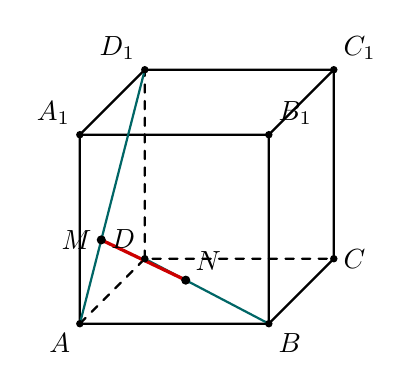
\begin{tikzpicture}[line join=round, line cap=round, >=Stealth, font=\normalsize, scale=0.75]
\coordinate (A) at (0,0);
\coordinate (B) at (3.2,0);
\coordinate (D) at (1.1,1.1);
\coordinate (C) at ($(B)+(D)-(A)$);
\coordinate (A1) at (0,3.2);
\coordinate (B1) at ($(B)+(A1)-(A)$);
\coordinate (D1) at ($(D)+(A1)-(A)$);
\coordinate (C1) at ($(C)+(A1)-(A)$);

\draw[thick] (A)--(B)--(C)--(C1)--(D1)--(A1)--cycle;
\draw[thick] (B)--(B1)--(C1);
\draw[thick] (A1)--(B1);
\draw[dashed, thick] (A)--(D)--(C);
\draw[dashed, thick] (D)--(D1);

\draw[thick, teal!80!black] (A)--(D1);
\draw[thick, teal!80!black] (B)--(D);

\coordinate (M) at ($(A)!0.33!(D1)$);
\coordinate (N) at ($(D)!0.33!(B)$);
\draw[very thick, red!80!black] (M)--(N);

\fill (A) circle (1.8pt) node[below left] {$A$};
\fill (B) circle (1.8pt) node[below right] {$B$};
\fill (C) circle (1.8pt) node[right] {$C$};
\fill (D) circle (1.8pt) node[above left] {$D$};
\fill (A1) circle (1.8pt) node[above left] {$A_1$};
\fill (B1) circle (1.8pt) node[above right] {$B_1$};
\fill (C1) circle (1.8pt) node[above right] {$C_1$};
\fill (D1) circle (1.8pt) node[above left] {$D_1$};
\fill (M) circle (2.2pt) node[left] {$M$};
\fill (N) circle (2.2pt) node[above right] {$N$};
\end{tikzpicture}%
}
\end{minipage}

\item Một nhóm bạn trẻ tổ chức dã ngoại đã dựng một chiếc lều có dạng hình chóp lục giác đều $S.ABCDEF$ với đáy là lục giác đều $ABCDEF$. Vào buổi tối, nhóm bạn muốn trang trí lều bằng một sợi dây đèn led quấn vòng quanh bề mặt các mặt bên của lều, bắt đầu từ đỉnh $A$ của đáy, quấn quanh lều qua tất cả các cạnh bên và kết thúc tại trung điểm $M$ của cạnh bên $SA$. Biết rằng tất cả các cạnh bên của lều đều dài $2\text{ m}$ và góc ở đỉnh của mỗi mặt bên là $\widehat{ASB} = \widehat{BSC} = \dots = 20^\circ$. Chiều dài ngắn nhất của sợi dây đèn led bằng bao nhiêu mét? \textit{(Làm tròn kết quả đến hàng phần mười.)}
\end{enumerate}

\begin{center}
\textbf{---------- HẾT ----------}
\end{center}

\end{document}
